\section{Research}
  I will now explore research done relating to the project specified. This will outline some design decisions that were made and link to other 
  sections of the report where they may be explored more. This section will explore parallelism and thread safety focusing on data stores as well as 
  CI/CD, it's pros and cons when deploying to live systems and how we as a team worked around it.

  \subsection{Storage Solutions and Parallelism}
  \label{sec:storageSolutions}

  Currently the schedule pipeline consists of two components, the ingester, followed by the schedule generator. The first part of this pipeline is
  parallelised, multiple lambdas can be ran at the same time to insert data into the redis. This is a harder task for the schedule generator to do,
  as it needs update a list of linked schedules to an episode in the redis store. This data can be edited through multiple streams, both the schedule
  catalogue pipelines, meaning the array could easily become incorrect/polluted. Sharing memory in a threaded/parallelised system is a well known 
  challenge and you need to know when it's safe to update/edit this memories value (https://homes.cs.washington.edu/~djg/teachingMaterials/spac/sophomoricParallelismAndConcurrency.pdf).
  This is also known as being thread safe which can be described as \textit{'different threads can access the same resources without exposing erroneous 
  behavior or producing unpredictable results'} (Ugarte, 2024).

  \begin{figure}[H]
    \centering
    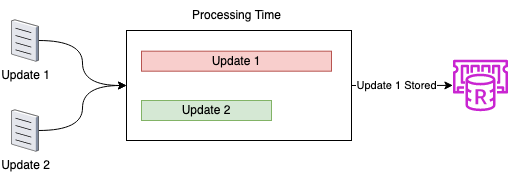
\includegraphics[width=6cm]{assets/raceCondition.drawio.png}
    \caption{Diagram showing how a broadcast list of an episode can become incorrect/polluted.}
    \label{fig:raceCondition}
  \end{figure}

  \subsubsection{Redis and Elasticache}
  We use amazons Elasticache (Amazon Web Services, 2024f) for our redis (REmote DIctionary Server) solution as it stores data in memory, which makes it 
  really quick to retrieve stored data (IBM, 2024). This is vital for us as we store large documents that need to be retrieved and sent to partners on 
  an API request. Redis is single-threaded but supports concurrency, \textit{'when at least two threads are making progress'} (Oracle Corporation, 2010) 
  which is not the same as parallelism, \textit{'when at least two threads are executing simultaneously'} (Oracle Corporation, 2010).

  \begin{figure}[H]
    \centering
    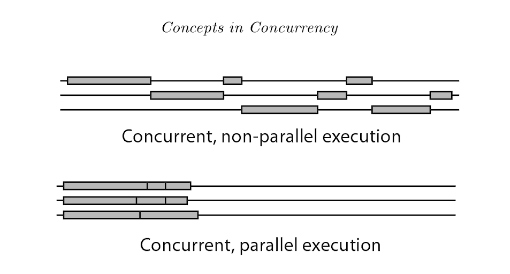
\includegraphics[width=8cm]{assets/concurrecnyVsParallelism.jpg}
    \caption{Difference between concurrency and parallelism. \url{https://books.google.ie/books/about/Introduction_to_Concurrency_in_Programmi.html?id=J5-ckoCgc3IC&redir_esc=y}}
    \label{fig:concurrecnyVsParallelism}
  \end{figure}

  This concurrency allows redis to support multiple requests at once, but it cannot do multiple operations at once; although more recent versions are allowing
  some safely threaded operations such as deleting records (Redis Ltd, 2024a). It also supports batch uploading and blocking commands, however these also 
  don't help keep the data thread-safe.

  \begin{itemize}
    \item \textbf{Pipelining} - Pipelining sends a block of commands at once, however does not guarantee that commands sent are done in sequence 
    (Redis Ltd, 2024b).
    \begin{figure}[H]
      \centering
      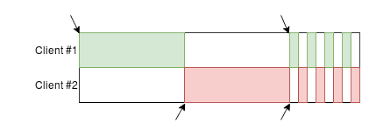
\includegraphics[width=8cm]{assets/pipelineOrdering.png}
      \caption{How redis pipelines don't guarantee sequential execution (Eyng, 2019).}
      \label{fig:pipelineOrdering}
    \end{figure}
    \item \textbf{Transactions} - Transactions are very similar to pipelines, however guarantee that the transactions commands are not interrupted by another
    clients requests and are therefore executed in sequence (Redis Ltd, 2024c).
    \item \textbf{Blocking Actions} - Blocking actions stop the current client from executing commands until the blocking action is complete. However other 
    clients can still send requests to the server whilst this client is blocked (Redis Ltd, 2024d). 
  \end{itemize}

  The options above still allow the previous race condition to occur, as instances of the schedule generator may vary in processing time and therefore the 
  time of writing to the redis cannot be guaranteed to be in order of the events.

  \subsubsection{How thread-safety can be achieved}
  When researching and spiking (Visual Paradigm, 2024) the project, other technologies were found that could help offer thread safety whilst parallelising
  the schedule generator. These were types of store/database locking mechanisms.

  \begin{itemize}
    \item \textbf{Pessimistic Locking} - This method \textit{'assumes that access to shared memory will be contended'} (Weston, 2011) and
    acquires a lock on the data to be edited. Any other client/connection attempting to edit this data must wait until this lock is released to update
    the data (Thornton, 2001). This can lead to issues such as deadlock which is when two clients are both awaiting on another clients lock to 
    be released. This can end up with both clients being stuck in a endless cycle of waiting for each other (Thornton, 2001; Apache Software Foundation, 2013).

    \begin{figure}[H]
      \centering
      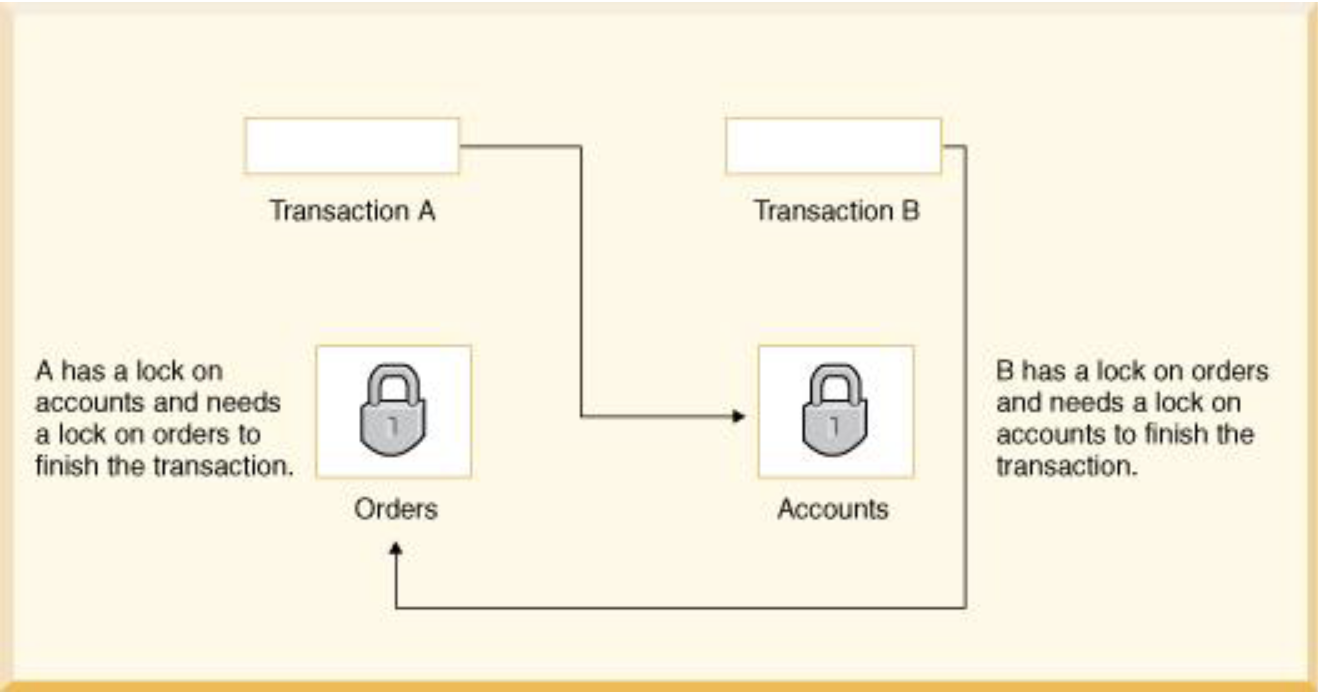
\includegraphics[width=8cm]{assets/deadlock.png}
      \caption{Example of a deadlock scenario (Apache Software Foundation, 2013).}
      \label{fig:deadlock}
    \end{figure}

    There is also a situation where a client locks a piece of data and for one reason or another halts, this would cause needless delay, when a timeout is 
    specified, if a timeout is not specified then this object would be locked from changes indefinitely (Thornton, 2001).

    \item \textbf{Optimistic Locking} - This method \textit{'relies on end-of-transaction validation'} (Graefe, 2016) and takes the outlook of presuming
    it's safe to write until the very end (Kanungo, Morena, 2023). Unlike its counterpart (pessimistic locking) it does not lock the record that is 
    being updated. Instead before the new data is written, the original data is checked against the current data stored (Thornton, 2001). If this data doesn't
    match then a change has occurred during processing and the new data to be written must be re-calculated with the new changes.

    \begin{figure}[H]
      \centering
      \includegraphics[width=6cm]{diagrams/sequence/Optimistic Locking.png}
      \includegraphics[width=6cm, height=6cm]{diagrams/activity/Optimistic Locking.png}
      \caption{Sequence and activity diagrams outlining logic of optimistic locking.}
      \label{fig:optimisticLocking}
    \end{figure}

    This above logic could be implemented into our redis solution. It would require either a total comparison of the object or a simple \textit{version}
    field that specifies when the object has changed.
  \end{itemize}

  During this investigation DynamoDB (Amazon Web Services, 2024e) was highlighted as a potential option due to it supporting optimistic
  locking. The final decision was to not use it however and stick with the current solution as there was a want to get the project started to keep 
  up with our roadmap and not further investigate this option. There was also more unknowns with this technology as we had never used it before.
  I will discuss a solution using DynamoDB in the \hyperref[sec:future]{\textbf{Future Work}} section of this report.
   
  \subsection{Agile and CI/CD}
  \label{sec:cicd}

  As a team we follow an agile approach to software development, more accurately we follow a kanban approach. The kanban methodology 
  \textit{'focuses more on monitoring and improving workflows'} (Heil, C, 2022) and doesn't use concepts such as sprints from scrum (Rehkopf, 2024). 
  Instead software created using the kanban approach is deployed/released when it's done (Rehkopf, 2024) and uses a kanban board where tickets move 
  across columns depicting where they are currently at in development cycle (Mauvius Group Inc, 2021).

  \begin{figure}[H]
    \centering
    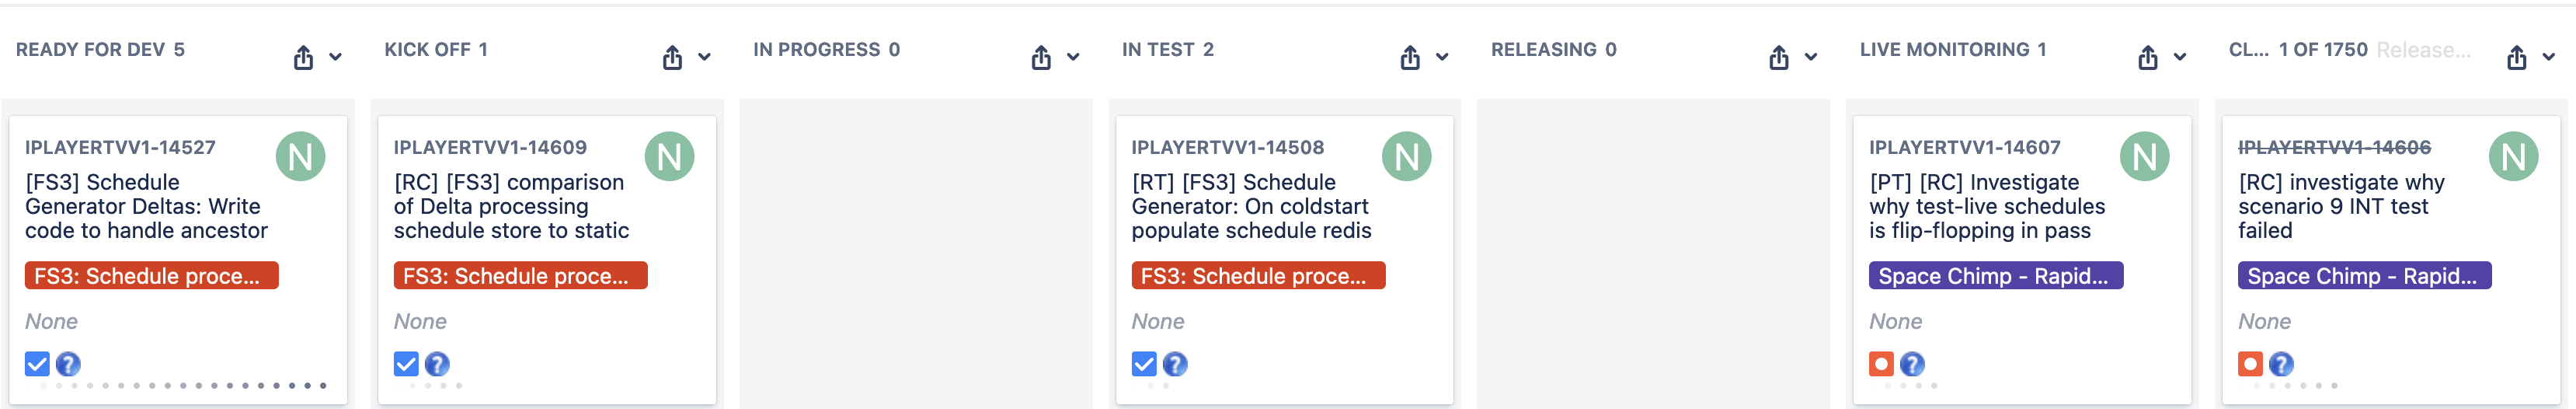
\includegraphics[width=10cm]{assets/kanbanBoard.png}
    \caption{SpaceChimps kanban board.}
    \label{fig:kanbanBoard}
  \end{figure}

  This workflow fit's in well with Continuous Integrations and Continuous Deployment (CI/CD). As a team we release/build all our own code to 
  multiple environments using Jenkins declarative pipelines (Jenkins, 2024).

  \begin{figure}[H]
    \centering
    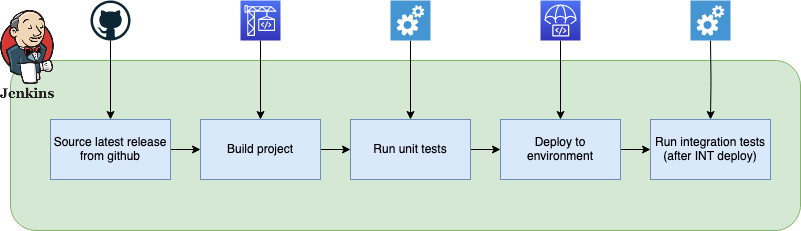
\includegraphics[width=10cm]{assets/pipeline.drawio.png}
    \caption{General pipeline flow.}
    \label{fig:pipeline}
  \end{figure}

  Having these well defined deployment pipelines makes deploying new code easy and helps manage deployments across multiple environments as configuration 
  can be built in to the pipeline (Rodriguez, et al, 2016). This approach allows bugs to be caught faster than when using 
  a \textit{'big-bang'} approach, as the bug is likely to be with a single new change (Department of Defence, 2021).
  The additional testing also gives more confidence in the code deployed and rollbacks are made extremely simple due to version control management.

  \vspace{0.2cm}

  There are of course some downsides to CI/CD, whenever an external platform, Jenkins in our case, is being used this opens up a new attack vector (NSA, 2023).
  OWASP keeps a list of some of these threats (OWASP Foundation, 2023), however they mostly comprise of poor 
  authentication to CI/CD systems and attacks by people who already have access to source code and the CI/CD platform itself (employees).

  Other issues include maintenance of the pipelines code/infrastructure and potential complexity (Wikström, 2019),
  this can be especially true when pipelines call other processes. 

  Code quality can become an issue, with technical debt increasing due to the encouraged continuous deployment of new software (Rodriguez, et al, 2016) 
  and more bugs also appear to occur. One study showed that the number of bugs actually increased when using CI/CD (Fairbanks, Tharigonda, Eisty, 2023).

  \begin{table}[H]
    \centering
    \begin{tabular}{|p{0.3\textwidth}|p{0.15\textwidth}|p{0.15\textwidth}|}
      \hline
      & CI/CD & No CI/CD \\ \hline
      Github average issues & 135.38 & 57.33 \\ \hline
      Gitlab average issues & 52.04 & 17.68 \\ \hline
    \end{tabular}
    \caption{Table from study showing difference in issues found between approaches (Fairbanks, Tharigonda, Eisty, 2023).}
  \end{table}
  
  However this same study also showed a commit velocity increase of 141\%, so it could be argued that these bugs are quickly remedied due to this quicker 
  release time. In addition to this as a team we do pull requests, another developer checks new code before release, which should also mitigate some 
  of the outlined issues above.

  \subsubsection{Software Changeover Strategies}
  The system that is being upgraded is in LIVE use by partners, but the work itself will take time to implement. We don't want to make changes to how
  the LIVE system works for partners but we do want to test that the new software works on the LIVE environment without a \textit{big-bang} deployment.

  There are three main types of changeover strategy, direct (big-bang), parallel running or a phased strategy and it's multiple variants (Banerjee, 2017). 
  
  \begin{figure}[H]
    \centering
    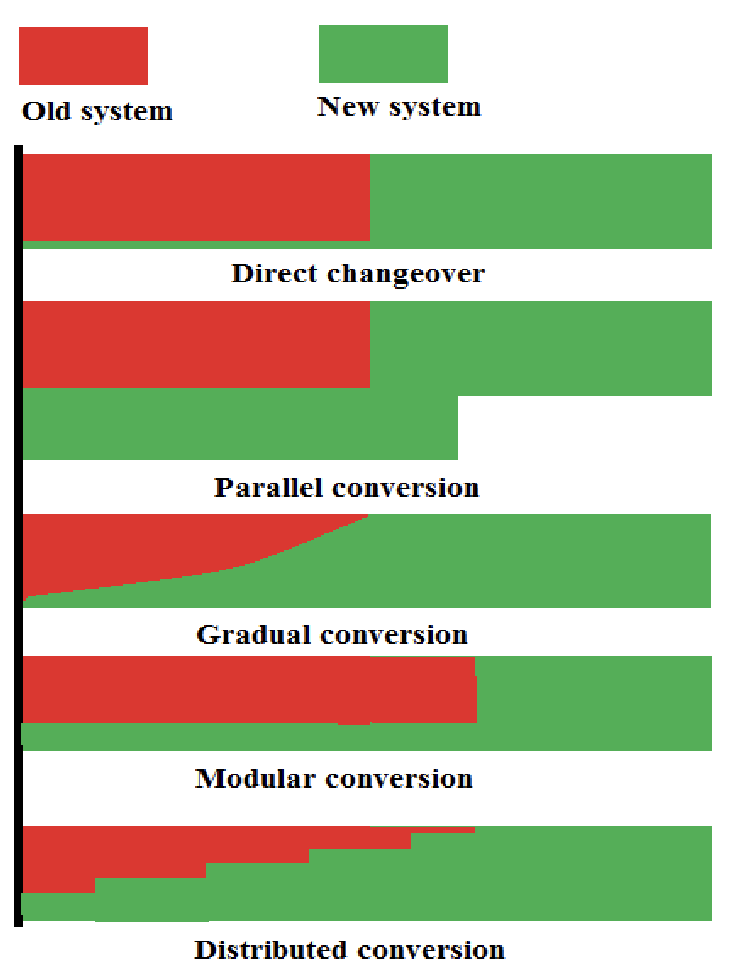
\includegraphics[width=6cm]{assets/changeoverStrategies.png}
    \caption{Timeline of different changeover strategies (Banerjee, 2017).}
    \label{fig:changeoverStrategies}
  \end{figure}
  
  As discussed a direct approach is risky and could easily run into errors, a phased approach in this situation is also not valuable as the we want 
  to remain consistent in the data we provide to all our partners, so a parallel system is our best option. Temporarily the old and new system will 
  run side-by-side, this will allow us to write comparison tests between the old output and the new (Smyth, 2020).

  In addition to having both systems the data on redis also needs to be separate as they may differ during development. This will be achieved by 
  using different redis keyspace prefixes (IoRedis, 2024) to keep the data separate and allow a test to check both for differences (Rustagi, 2023). 
  The partners would continue to get data from the old keyspace, when we are happy with our comparison tests the partners can be swapped over to the new 
  keyspace and the old data can be deleted. 

\newpage